\section{Geomorfolog\'{i}a.}
La geomorfolog\'{i}a de la zona de estudio se presenta en la figura \ref{fig:mapageomorfo}, est\'{a} caracterizada principalmente por laderas con 23\% de pendiente con desviaci\'{o}n est\'{a}ndar del 10\%.
Seg\'{u}n se describe en (memoria gologica) la zona presenta una fuerte influencia estructural lo cual se refleja en abundante fallamiento y plegamiento, de ah\'i que la expresi\'{o}n morfol\'{o}gica de la zona exhiba laderas de pendiente media a larga con pendientes de inclinaci\'{o}n abrupta. En la Ladera norte de la Qda. La Linda se presenta un patr\'{o}n de drenaje subdendr\'{i}tico, por lo cual se clasifica esta unidad como un Gancho de Inflexi\'{o}n (Sgf), mientras que en la ladera sur el patr\'{o}n de drenaje es Subparalelo, por lo cual la unidad se caracteriza como un Espol\'{o}n Moderado de longitud larga (Sesml).\par
Ambas laderas muestran cicatrices de movimientos en masa tipo rotacional, adicionalmente se presentan movimientos tipo traslacional en el Sesml. 
 \textbf{revisar las definiciones de cada unidad}\par


\begin{figure}[H]
\centering

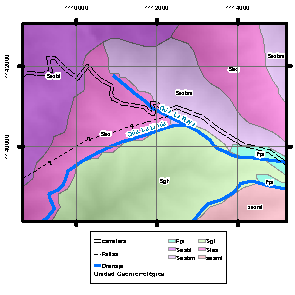
\includegraphics[width=.8\textwidth]{img/geomorfo.pdf}
\caption{Mapa geomorfol\'{o}gico. Basado en (mapa geomorfo). Acercamiento elaboraci\'on propia}

\label{fig:mapageomorfo}
\end{figure}